\documentclass{book}

\usepackage{mathpazo}
\usepackage{natbib}
\usepackage{makeidx}
\usepackage{xcolor}
\usepackage[bookmarks]{hyperref}
\usepackage{showidx}
\usepackage{aas_macros}
\usepackage{graphicx}

\makeindex
\newcommand\fakeplot{%%
  \fbox{\rule{1in}{0pt}Plot placeholder \rule{1in}{0pt}\rule{0pt}{2in}}}


\begin{document}

\begin{titlepage}
\begin{center}
  \vfill
  
  {\LARGE \textsc{Practical Cosmology}}

  \vfill
    \vfill

  Kevin M. Huffenberger
  \vskip 1 ex 
  Department of Physics \& Astronomy \\
  Mitchell Institute for Fundamental Physics \& Astronomy \\
  Texas A\&M University
  \vfill

  \vfill
  \vfill
  
  $\copyright$ 2026 KMH
\end{center}

\end{titlepage}

\section*{Preface}

We are making vast improvements in our knowledge of the Universe via the acquisition of precision data, and understand that we live in a vast and complicated universe about which we only understand the general outlines.  The normal matter that we understand through the standard model of particle physics makes up only five percent of the contents of the universe.  The dark matter and the dark energy are distinctive substances; their  properties are exotic and not well understood.  We study the brightness of supernovae, the fluctuations in the temperature and polarization of the cosmic microwave background, the clustering of galaxies, the abundance of primordial nuclei, and other observations.   Students and researchers working in cosmology should have a background in the theory underlying the cosmological models, and most cosmology textbooks focus on these theoretical aspects.  They also need a deep understanding of the observations and the statistics computed from the data to make comparisons to the theoretical models.  This text addresses the second need.

The two tasks are somewhat different.  For example, the computation of the theoretical power spectrum of the cosmic microwave background requires a detailed and complicated computation using perturbation theory in general relativity, but the processing of a CMB measurement to get a data power spectrum to compare to that theory requires no general relativity at all.  Indeed, in this book, there is little general relativity past the first chapter, and not much there either.  Instead the reader will find probability, statistics, Monte Carlo sampling, harmonic transforms, filters, and signal processing techniques.  These are some of the practical tools for measuring the details of our Universe.

\section*{Acknowledgments}
I thank
Peter Brown
and
Nao Suzuki
for useful scientific discussions.
Student readers who helped find typographic errors and other problems include:
George Fagan,
Aaron Hughes,
Sophia Paulino Korte,
Mason Moenter,
and
Annabella Yang.
\textcolor{red}{More acknowledgments...}


\tableofcontents

\chapter*{Introduction}

The universe is vast and old and dynamic.  We know that the time since the Big Bang may be $\sim 13.8$ billion years, although we are a few percent uncertain because we are still trying to understand the Universe's present-day expansion rate, and our knowledge of the age depends on that.  A photon or graitational wave traveling at light speed from the time of the Big Bang and just arriving here now would have come from a point in space that is today 46.3 billion light years away.  This number is bigger than 13.8 billion light years because the Universe has expanded in the meantime.  

We have some remarkable facts to start with.
\begin{enumerate}
  \item On large scales, $>1$ gigaparsecs (Gpc), the universe at the present day consists of a uniform sea of galaxies, stretching in all directions.
  \item On average, these galaxies move apart (as observed in Doppler-shifted light).  We interpret this as the whole spacetime expanding.
  \item Under the rules of general relativity, we can model the {scale factor} of the universe as a function of time, telling us how the spacetime.  Amazingly, the scale factor approaches zero a finite time ago, which is what we mean by the time of the Big Bang.
\end{enumerate}

Noting that the universe appears to be \textbf{homogeneous} (uniformly the same in every location) and \textbf{isotropic} (the same in every direction), we assume the ``cosmological principle'' that we are not at a special location.  This we mean in a statistical sense; the Earth is different from a star or the vacuum of outer space, but on a similar planet in a similar galaxy, a similar creature could study cosmology, and that creature would draw the same conclusions as us.  Because the universe is homogeneous and changing in time, we first need to study uniform but dynamic spacetimes.

\textcolor{red}{Describe the contents of each chapter in turn}

\chapter{Cosmology basics}

\section{Flat and curved spaces}
Cosmology is the study of the universe on the large scales, so we need to spend some time understanding how we are going to quantify and label positions in space and time.  Already in physics, we are used to labeling points in space with coordinates like $(x,y,z)$ or $(r,\theta,\phi)$.  We are also accustomed to computing the distances between points, especially in cartesian coordinates.

We know that the distance between two points can be computed from the coordinate differences via
\begin{equation}
  \Delta \ell = \sqrt{(\Delta x)^2 + (\Delta y)^2 + (\Delta z)^2 }.
\end{equation}
For infinitesimally small changes in the coordinates, we could write $  (d\ell)^2 = (dx)^2 + (dy)^2 + (dz)^2$, and use that to figure our the length of a curved path.  That equation is called the \textit{line element}\index{line element} and expresses the \textit{metric}\index{metric} of the space: it tells us how to measure distance.  For example, if a path traces out coordinates $x(\lambda),y(\lambda),z(\lambda)$ as a function of some parameter $\lambda$, we can measure the length with the integral
\begin{equation}
   \ell = \int_{\lambda_{\rm start}}^{\lambda_{\rm finish}} d\lambda \sqrt{ \left(\frac{dx}{d\lambda} \right)^2 + \left(\frac{dy}{d\lambda}\right)^2 + \left(\frac{dz}{d\lambda}\right)^2}.
\end{equation}
We recognise that this is the right integral to use whether or not we are actually trying to evaluate it.

We also could change the coordinates that we use to define the space and trace out any given path.  For example, a Euclidean space in spherical polar coordinates has a metric
\begin{equation}
   d\ell^2 = dr^2 + r^2 d\theta^2 + r^2 \sin^2 \theta d\phi^2.
\end{equation}

We learn in special relativity that we need also to label event with space and time coordinates $(t,x,y,z)$, which is simple enough.  The surprise is that we further learn that different observers will disagree on the measurements of distances and time intervals, but all observers will agree on the spacetime interval between two events.  It is invariant.  The spacetime interval could be written as
\begin{equation}
  (\Delta s)^2 = -(\Delta t)^2 +  (\Delta x)^2 + (\Delta y)^2 + (\Delta z)^2
\end{equation}
which is a little weird but at least the space follows the familiar rules of Euclidean geometry.  The relationship between the three space coordinates, the one time coordinate, and the spacetime interval is called the spacetime metric.  The time coordinate $t$ is the wristwatch time of an observer but will not synchronize with the wristwatch time of an observer in a different frame, one that moves with nonzero constant relative velocity.  We are going to measure time in units of length so that the units of the equation work out, thus taking the speed of light $c=1$.  For example, a time interval of $\Delta t = 1\,\mbox{m} = 1\,\mbox{m}/c = 3.3\times10^{-9} s$.

Our footing gets much less steady when we turn to general relativity, which is needed to treat accelerations and provides our best understanding of the physics of gravity.  In general, the space does not need to be Euclidean, so our common rules, such as ``the sum of angles in a triangle is $180^\circ$,'' might not be true.  Further, the numbers that we assign as coordinates to points in space are just labels, and (within some limits) we have enormous freedom to choose how we assign the coordinates.  (Some choices are more suitable than others.)  Like in special relativity, the spacetime interval along a path in the spacetime is invariant.

\begin{figure}
  \caption{Diagram of a 2-d spherical surface in cartesian coordinates.}
\end{figure}

We don't even need to get relativity to get experience with coordinates in curved spaces.  We can describe the 2-d surface of the sphere, a surface with $x^2 + y^2 + z^2 = R^2$, in polar coordinates.  Let $R$ be the radius of the sphere, $r$ be the cylindrical distance from polar axis to a point on the sphere and $\phi$ be the azimuthal angle of that point to the $x$-axis.  It is not too much trouble to show that the length of a path along the surface from the north pole to a point is 
\begin{equation}
  \ell_{\rm radial} = \int_0^r \frac{dr'}{\sqrt{1-r'^2/R^2}} = R \sin^{-1}(r/R) > r. \label{eqn:2d_sphere_path_radius}
\end{equation}
So confined to the space (i.e.\ the surface), $r$ is the coordinate away from the origin but not the distance from the origin, which is larger.
We can also consider a circular path with a fixed radius around the whole sphere, which has length
\begin{equation}
  \ell_{\rm circumference} = \int_0^{2\pi} d\phi r = 2\pi r.  \label{eqn:2d_sphere_path_circumference}
\end{equation}
So that circle, considered along the curved surface only, has more radius than you would expect given the circumference.  This is a manifestation of the surfaces positive curvature.  Also note that that point with $r=0$ is not a special point of the sphere.  All points are the same because, mathematically, a sphere is homogeneous and isotropic, so we could have defined that origin point anywhere. From Eqns. (\ref{eqn:2d_sphere_path_radius}) and (\ref{eqn:2d_sphere_path_circumference}) we can work out that the metric for the surface of the sphere is
\begin{equation}
  dl^2 = \frac{1}{1-r^2/R^2} dr^2 + r^2 d\phi^2
\end{equation}
A sphere with a very large radius $R$ compare to the coordinate $r$ values of interest looks pretty flat, and that is reflected in the metric.

For a 2-d hyperbolic surface that satisfies $x^2 + y^2 - z^2 = R^2$ possesses a similar metric, differing only in the sign of the addition in the denominator of the radial term,
\begin{equation}
    dl^2 = \frac{1}{1+r^2/R^2} dr^2 + r^2 d\phi^2,
\end{equation}
and is also a homogeneous and isotropic space, but has less radius than you would expect for a given circumference, compare to a flat plane.

These are both two-dimensional surfaces that we have embedded in three-dimensional Euclidean space.  We can go to one higher dimension, looking at surfaces that satisfy $x^2 + y^2 + z^2 \pm u^2 = R^2$.  These spaces work basically the same and we unsurprisingly find a metric with
\begin{equation}
  d\ell^2 =  \frac{1}{1-kr^2/R^2} dr^2 + r^2 d\Omega^2
\end{equation}
where the solid angle $d\Omega^2 = d\theta^2 + \sin^2 \theta d\phi^2$, and the parameter $k$ is $+1$ for a spherical space and $-1$ for a hyperbolic space.  We can also include the value $k=0$ to recover normal 3-d spherical polar coordinates.  Notice that all of the metric weirdness is in the radial coordinate.  The angular part of the metric looks pretty normal, so the formulas for the radius of a circle is still $2\pi r$ and the surface area of a sphere is still $4\pi r^2$, but you have to be a little careful about what you mean by $r$.

\section{Cosmological FRW metric}
For much of practical observational cosmology, we will not need much general relativity, but a few results are crucial.  As noted before, we observe that the universe is statistically homogeneous and isotropic, meaning that at different locations and in different directions, the universe is basically the same: composed of galaxies of the same various types, oriented in all different directions at random.  Also true is that the universe is not static, but dynamic; it changes in time.  When we look at the most distant galaxies, where the light has taken many billions of years to reach us, the galaxies are different, forming stars alternatively less then more then less vigorously.  Older galaxies have more pristine gas with fewer heavy elements.  Moreover, the light from distant galaxies is \textit{redshifted}\index{redshift}, or shifted to longer wavelengths, which is strong evidence that the universe is expanding in time, as we will see.

In general relativity, these conditions end up being quite restrictive.  The metric that describes how to measure spacetime intervals in homogeneous, isotropic, dynamic spacetimes can be written as
\begin{equation}
  ds^2 = -dt^2 + a^2(t)\left[ \frac{dr^2}{1 - kr^2/R_0^2} + r^2 d\Omega^2  \right]
\end{equation}
where $r$ is a radial coordinate (called a comoving coordinate) but again is slightly different to what we are used to, and $\theta$ and $\phi$ are angular coordinates that work normally.  This metric is extremely important.  The parameter $k$ denotes the three different kinds of spacetimes that are allowed by our restrictive conditions.  Values $k = \{ -1, 0, +1 \}$ mean that the space has negative curvature, is spatially flat, or has positive curvature.    All of this is familiar from our discussion of curved spaces above.

The new element is the function $a(t)$, which is called the \textit{scale factor}\index{scale factor} and specifies how the size of the universe changes over time.  By convention, we set $a(t_{\rm now}) = 1$, which means that the comoving coordinate refers to the present time. Similarly, the parameter $R_0 > 0$ is the radius of the curvature of the space at the present day, but the curvature scale at other times grows or shrinks according to $a(t)$.  The meaning of $t$ is the wristwatch time of ``co-moving'' observers.  By comoving, we mean these are observers who are carried along with the expansion of the universe, and their relative motions are determined only by the expansion.  They have no independent motion (that is, peculiar velocity\index{peculiar velocity}).

We call this metric the Friedmann-Robertson-Walker (FRW) or Friedmann-Lemaitre-Robertson-Walker (FLRW) metric after the people who found and worked with it first.  We have measured the spatial curvature and know that the radius of curvature exceeds $R_0 > ???$ (at 95\% confidence in Planck satellite data), so our universe is fairly flat.  In some cases we will restrict to that case.  Cosmology is concerned with the very largest size scales in the universe.  We are essentially stuck in one spot, in the Milky Way, so we can call our position as the origin of our coordinate system. 

The expansion rate at any time is given by the time derivative of the scale factor.  This is typically rescaled by the scale factor itself to give the \textit{Hubble parameter}\index{Hubble parameter},
\begin{equation}
  H = \frac{1}{a} \frac{da}{dt}. 
\end{equation}
The present-day expansion rate is called the \textit{Hubble constant}\index{Hubble constant},
\begin{equation}
  H_0 = H(t_{\rm now}) = \dot a(t_{\rm now}) \approx \frac{70\,\mbox{km/s}}{\mbox{Mpc}} \approx 2.3\times 10^{-18}\,\mbox{s}^{-1}.
\end{equation}
All determinations of distance depend on the Hubble constant; it is an enormously important quantity and there is still some few percent uncertainty in its value.  The inverse of the Hubble constant can be expressed as a time, about 240 Myrs, or a distance, about 4.2 Gpc.
  
In flat space (k=0), the physical distance (like you would measure with a ruler) from the origin to a point depends on the comoving coordinate as
\begin{equation}   
  \ell_{\rm phys} = a(t) r 
\end{equation}
while the physical velocity of an object is
\begin{equation}
  v_{\rm phys} = \frac{d(\ell_{\rm phys})}{dt} = \frac{da}{dt} r + a \frac{dr}{dt} = \frac{\dot a}{a} a r + a \frac{dr}{dt} = H \ell_{\rm phys} + v_{\rm pec}
\end{equation}
The first term in the velocity is called the \textit{Hubble flow}\index{Hubble flow} and the second term is called the \textit{peculiar velocity}\index{peculiar velocity}.  The Hubble flow is the velocity that you measure from the expansion of the Universe.  Nearby, where the Hubble parameter is close to the present-day value, we find that galaxies tend to move away from us at around 70 km/s per Mpc of distance away.  The peculiar velocity is the independent velocity of a galaxy is typically around 1000 km/s, so we need to look further than tens of Mpc for the Hubble flow to dominate the overall velocity of an object.  In practice, we measure the \textit{cosmological redshift}\index{redshift}, $z$, of the spectral lines of an object compared to the wavelength of emission.
\begin{equation} 
  \lambda_{\rm obs}/\lambda_{\rm em} = a(t_{\rm now}) / a(t_{\rm em}) = 1+z
\end{equation}
We have $z=0$ at the present day, $z \sim 10$ when the first stars and galaxies are forming, and $z =1100$ when the CMB is released.  The wavelength is expanded, but since the speed of light is constant, the frequency of light slows, as does the observed rate of any other process.  Thus energy and momentum of photons (and other objects) drops as the Universe expands.  Energy conservation is the result of the symmetry of time-invariance.  The spacetime of an expanding universe is not time invariant, so we cannot expect energy conservation.  As the momentum of objects redshifts away, they over time lose their peculiar velocity and come to join the Hubble flow.

\section{Friedmann equations and model universes}
Much of the development of the universe clearly depends on the \textit{expansion history}\index{expansion history}, the scale factor as a function of time: $a(t)$.  Treating the universe the as a uniform fluid, the Einstein equations of general relativity yield two differential equations that relate the scale factor to the energy density and pressure of the Universe: the first Friedmann equation,
\begin{equation}
  H^2 = \left( \frac{\dot a}{a} \right)^2 = \frac{8\pi G}{3} \rho - \frac{k}{a^2 R_0^2}, \label{eqn:friedmann1}
\end{equation}
and the second Friedmann equation
\begin{equation}
  \frac{\ddot a}{a} = -\frac{4 \pi G}{3} (\rho + 3 P) \label{eqn:friedmann2}.
\end{equation}
Examining the first Friedmann equation we see that the expansion rate on the left and contributions from the density and the curvature on the right side.

\subsection{Components of the Universe}
We need to describe these types of matter and radiation in the Universe that contribute to the Friedmann equations.  We also need to understand how the densities change with the scale factor, which allows us to solve for $a(t)$.  We do not have energy conservation but do have a continuity equation
\begin{equation}
  \dot \rho + 3 \frac{\ddot a}{a}(\rho + P) = 0
\end{equation}
We often consider a proportional relationship between pressure and density, the \textit{equation of state}\index{equation of state} with equation of state parameter $w$ as the constant of proportionality,
\begin{equation}
  P = w \rho.
\end{equation}
This allows us to solve the continuity equation to relate density to the scale factor of expansion.
\begin{equation}
  \rho \propto a^{-3(1+w)}
\end{equation}

\paragraph{Matter.}  When we talk about \textit{matter}\index{matter}, we are refering specifically to non-relativistic particles for which the kinetic energy is small compared to the rest mass, and equivalently, the pressure is small compared to the density ($P \ll \rho$ in units where $c=1$).  Thus for $w=0$, the continuity equation provides
\begin{equation}\rho \propto a^{-3}.\end{equation}
This result makes sense.  The total density of matter is the particle rest mass times the number density, $\rho_m = mn$, and the number density of particles is diluted by the expansion of the universe as $n \propto a^{-3}$.

Our universe includes at least two categories of matter.  The normal matter\index{matter!normal} consist of the types that we are most familiar with on Earth: proton, neutrons, nuclei, atoms.  In the late universe, there are dense object like planets and stars, but even today the bulk of the normal matter is in the form of diffuse gas or plasma.  This component is also sometimes given the catchall term ``baryons.''  This component does have some pressure, which is important for driving acoustic oscillations in the CMB, but even at that time and ever since, the bulk of the baryons were non-relativistic, so the pressure was not important in determining their contribution to the expansion history.

The second category of matter, \textit{dark matter}\index{matter!dark}, is a substance of unknown type that contributes about five times as much to the total density budget as normal matter.  It is unclear if this is a subatomic particle or something macroscopic.  We do not know if there is one type or multiple types that fill out an entire ``dark sector'' of particle physics.  There is so far no evidence for interactions between this component and photons or baryons.  As such this component seems to genuinely provide no pressure, and is usually modeled that way, although in actually there may be some interactions at very low level (which would be our main hope of discovering it in a particle physics detector).  Some models include weakly-interacting massive particles (WIMPs), axions (proposed particles to solve the strong CP problem in QCD), and primordial black holes.

\paragraph{Radiation.}  For both photons and any gas of relativistic particle, the pressure relates to the energy density as
\begin{equation}
  P_r = \frac{1}{3} \rho_r
\end{equation}
or $w=1/3$.
This in turn means that the energy density scales with expansion as
\begin{equation}
  \rho_r \propto a^{-4}.
\end{equation}
The expansion of the volume dilutes the photon number density while the energy per photon is redshifting away, thus $\rho \propto n E \propto a^{-3}a^{-1}$.

Included in radiation are photons, light particles (including neutrinos), and gravitons.  The light is predominantly the photons that at late times becomes the CMB.  These photons follow a thermal (Planck) blackbody spectrum and the redshift effect is the same as adjusting the temperature $T \propto a^{-1}$.

What we count as a light particle depends on when in the history of the universe we are talking about.  The total energy of a particle is $\gamma m$.  At early times the energy $E \sim kT$, but the scale factor is small and so the temperature is high.  Thus every particle is relativisitic if you go back early enough in the universe.  Radiation is the dominant contribution to the energy density early on.  Neutrinos are relativistic for the early history of the universe, and although we don't yet know all the neutrino masses, at least some neutrinos are massive enough to not be relativistic now.

Gravitons are massless particles and so are always relativistic, but they don't have much overall energy density and contribute negligably to the expansion history.

\paragraph{Dark Energy.}\index{dark energy}  In General Relativity, the Einstein equations are differential equations that relate the properties of spacetime on one side and matter-energy content on the other.  It is not uniquely determined and you can add a term proportional to the metric tensor without messing up the continuity equation for the stress-energy density.  Einstein originally introduced such a term, conventionally written as proportional to some constant number $\Lambda$, essentially asserting it as an innate property of spacetime.  He did this because it allows solutions to the equations that corresponded to the static universes he desired, ones unchanging in time.  (When the universe was found to be expanding, Einstein famously called this term his ``greatest blunder.'')

Another point of view is to consider what that term would mean if you moved it to the other side of the equation, mathematically equivalent, and considered it as a time of energy density.  It acts as a fluid with the equation of state
\begin{equation}
  P_\Lambda = -\rho_\Lambda,
\end{equation}
which has a positive energy density but a negative pressure.  The equation of state parameter is $w=-1$ and so
\begin{equation}
  \rho_\Lambda \propto a^0
\end{equation}
is constant.  The density of this component does not dilute with expansion of the universe.  This is very weird and  does not fit with our intuitions of how substances work.  However, current modeling requires this component, dubbed ``dark energy,'' to account for about 70 percent of our present-day energy budget.

This component is utterly mysterious to us.  It may ultimately be simply a property of spacetime, just a \textit{cosmological constant} in the equations of GR.  It may be an energy density associated with the vacuum.  This might make the density dependence on expansion more understandable.  An expanding volume produces more vacuum produces more dark energy.  In quantum mechanics, the (observed) Casamir effect depends on a sea of vitual particles and a zero-point energy associated with the vacuum.  However, a simple theory computation, accounting for the particles we know about predicts a vacuum energy value which is huge, a factor of $10^{60}$ greater than what we observe.  This is the unresolved \textit{cosmological constant problem}.

There are other models where the dark energy is one or more particle physics field and could be dynamic and not a constant after all.  This is an active area of research.

\subsection{Expansion histories of model universes}
With the $\rho(a)$ dependence of the of the different components, we can solve the Friedmann equations directly in simple cases.  For example, in flat universes that are dominated by a single component, we find for different equations of state 
\begin{equation}
  a(t) \propto \left\{
  \begin{array}{lll}
    t^{2/3(1+w)}  = \left\{ \begin{array}{l} t^{2/3}\\ t^{1/2} \end{array} \right. & \begin{array}{l} w=0  \\ w = 1/3 \end{array} &  \begin{array}{l} \mbox{matter-dom.}  \\ \mbox{radiation-dom.} \end{array} \\
    \exp(Ht) & \begin{array}{l}w = -1 \end{array}& \begin{array}{l} \Lambda\mbox{-dom.} \end{array}
  \end{array}
  \right. 
\end{equation}
There are several things to note about these solutions.  The matter and radiation solutions are increasing in size but decelerating (concave-down curves), and we understand this in terms of the attractive gravitational pull of all the matter in the universe slowing the expansion.  In a flat universe, however, it is not enough to arrest the expansion.

In a flat, cosmological-constant-dominated Universe, by contrast, the expansion is exponentially accelerating.  The Hubble parameter is always constant in this case.   We think that our universe today has mostly transitioned from being matter dominated to $\Lambda$ dominated, as the expansion dilutes the matter but not the cosmological constant.  The components had equal energy density about $z=0.3$.  The matter-dominated phase lasted about 10 Gyr.  Because of the density scaling with scale factor, prior to the matter dominated phase was a radiation dominated phase (equal components about $z=3400$).  The radiation dominated phases lasted only about 50 kyr.  Looking backward in time, both matter and radiation dominated universes reach zero size a finite time in the past.  This is the origin of the idea of the ``hot Big Bang.''  We think there was another epoch of exponential expansion prior to the radiation dominated phase.  This is \textit{inflation}\index{inflation} and we understand that even less than dark energy.

Because our Universe has multiple components, and curvature is always a possibility, we need to treat the solution for $a(t)$ more generally.  From the first Friedmann equation (\ref{eqn:friedmann1}), we see that for a particular expansion rate there is a particular \textit{critical density}\index{critical density} associated with flatness.  To have a flat ($k=0$) universe today ($a=1$, $H=H_0$), we must have
%\begin{equation}
%  H_0^2  = \frac{8\pi G}{3} \rho_{\rm crit,0} 
%\end{equation}
\begin{equation}
  \rho_{\rm crit,0}   = \frac{3 H_0^2}{8\pi G},
\end{equation}
a density that works out to be about one Milky Way-sized galaxy per cubic Mpc.  We do not see that much luminous matter, but the other components, dark matter and dark energy, make up the difference, leaving our Universe very close to flat.

We can cast the first Friedmann equation into a nice form by looking at the ratio of the density to the critical density for each component
\begin{equation}
  \Omega_i = \frac{\rho_{i,0}}{\rho_{\rm crit,0}}
\end{equation}
for $\Omega_r$, $\Omega_m$, and $\Omega_\Lambda$.
We can define an analogous quantity for curvature, 
\begin{equation}
  \Omega_k = \frac{-k/R_0^2}{H_0^2}   \qquad \mbox{or} \qquad R_0 = \frac{1}{H_0\sqrt{-\Omega_k / k}},
\end{equation}
but note the change in sign, so that $\Omega_k<0$ for positive curvature $k>0$.  With current limits on $|\Omega_k| < 0.005$, we know that $R_0 > 60$ Gpc.   With these, the Friedmann equation \ref{eqn:friedmann1} becomes,
\begin{equation}
  H(a)^2 = H_0^2 ( \Omega_r a^{-4} + \Omega_m a^{-3} + \Omega_k  a^{-2}+  \Omega_\Lambda ). \label{eqn:H_in_terms_of_Omega}
\end{equation}
Rearranging, we get a separable equation
\begin{equation}
\frac{da}{dt} = \dot a = H_0 (\Omega_r a^{-2} + \Omega_m a^{-1} + \Omega_k  +  \Omega_\Lambda a^2)^{1/2} = H_0 F(a),
\end{equation}
that can be integrated and inverted to give the functional relationship between $a$ and $t$,
\begin{equation}
  \int^1_a \frac{da'}{H_0 F(a')} =  \int^{t_{\rm now}}_t dt'.
\end{equation}

\textcolor{red}{Talk about the models and cosmological parameters.}

\begin{figure}
  \begin{center}
    \fakeplot
  \end{center}
  \caption{For the $\Lambda$CDM model, an annotated plot of $a(t)$ and $H(t)$, with $z$ on the other axis.  Maybe a time zoom to see matter radiation equality.}
\end{figure}

\textcolor{red}{include open vs closed models?}

$\Lambda$CDM model


These ``$\Omega$'' parameters are the first of what we will call \textit{cosmological parameters}\index{cosmological parameters}.  They determine how a specific cosmological model develops over time.  Much of the science of observational cosmology is dedicated to making measurements of observable quantities and using them to determine the values of the cosmological parameters within the model.






\section{Distance measures}

The redshift of objects is relatively easy to measure, directly provides the amount of expansion in the universe since that time, and gives us one measurement of the distance to an object.  We need to understand the relationship between redshift and the other observables that are also related to distance, most prominently the brightness and angular size of objects.  Brightness and angular size are also relatively easy to measure on the sky.  Comparisons of these observables and their associated distance--redshift relationship over cosmic time give us ways to constrain the cosmological model.

Important in the discussion of distances are the concepts of \textit{standard candles}\index{standard candle} and \textit{standard rulers}\index{standard ruler}.  A standard candle is an object of known luminosity that we can compare to its measured brightness to determine the distance.  The most well known standard candles are type Ia supernova.  These are sometimes referred to as standardizable candles since they are not all identical, and their luminosity is not known from first principals, but the luminosity can be well calibrated by a series of observations that we will describe in the next chapter.  A related concept is a standard siren\index{standard siren}, which is a gravitational wave source of known power that we can compare to the locally measured strain.  An example would be a binary black hole merger that is understood in such detail that the power is understood and localized such that the redshift of the host galaxy is measureable.

A standard ruler is object or feature of known comoving or physical size that we can compare to the measured angular size.  Examples of standard rulers are the baryon acoustic oscillations, or soundwaves in the primordial plasma, that are visible both as peaks in the CMB power spectrum and in the distribution of galaxies.  

We want to work out the distance to a point where some radiation was emitted.
\begin{equation}
  d\chi = \frac{dr}{(1 + kr^2/R_0^2)^{1/2}}
\end{equation}
which you can integrate to get
\begin{equation}
  r = S_k(\chi) = \left\{
  \begin{array}{ll}
    R_0 \sinh(\chi/R_o) &  k=-1 \\
    \chi & k=0 \\
    R_0 \sin(\chi/R_o) &  k=+1
  \end{array}
  \right.
\end{equation}
You can compare Eqn~(\ref{eqn:2d_sphere_path_radius}) to see that $\chi$ is the radial distance between points in the (possibly) curved space.  We call $\chi$ the comoving distance\index{comoving distance}.

Writing the FRW metric in terms of the comoving distance, we have
\begin{equation}
  ds^2 = -dt^2 + a^2 \left[ d\chi^2 + S_k^2(\chi) d\Omega^2 \right]
\end{equation}
Photons travel on null geodesics, paths with $ds^2 = 0$, so a photon on a radial path ($d\theta = d\phi = 0$) will have
\begin{equation}
  d\chi = \frac{dt}{a(t)} = - \frac{dz}{H(z)}
\end{equation}
where we have used the differential of $1+z = 1/a(t)$ in the last equality.  Integrating, we find
\begin{equation}
  \chi = \int_{t_{\rm em}}^{t_{\rm now}} \frac{dt}{a(t)} = \int_0^z \frac{dz'}{H(z')} 
\end{equation}
to get $\chi(t)$ or more usefully $\chi(z)$. As we see, this distance--redshift relation measures expansion history via the integrated $1/a(t)$ or $1/H(z)$.  Comparing Equation~(\ref{eqn:H_in_terms_of_Omega}), you can see that $\chi(z)$ has an amplitude determined by $H_0^{-1}$ and a shape determined by the the $\Omega$ parameters (the composition of the Universe).

The cosmology dependence comes from the cosmology's effect on the expansion history.

\begin{figure}

  \caption{Diagrams for different notions of distance, including $D_M,D_A,D_H$.}
  \label{fig:distances1}
\end{figure}


\paragraph{Comoving distance.}
As mentioned, we call $\chi$ the comoving distance.  It is the physical distance today if we were to measure with a ruler to the point where the emission previously came from.

\paragraph{Transverse comoving distance.}  This also sometimes called the metric distance and people often use the symbol $D_M$.  This is the distance used to compute an arc length \textit{as measured today}, so we are not worried about the expansion of the universe.  So an arc with angle $\delta\theta$ and radius $\chi$ has an arc length $D_M \delta\theta$.  See Fig.~\ref{fig:distances1}.  We have already encountered this quantity, which has the value
\begin{equation}
  D_M(z) = S_k(\chi(z)) = r(z).
\end{equation}
finding that it is the same as the comoving coordinate.  In a flat universe only, this quantity is also the comoving distance $\chi$.

Suppose an object with physical size $\delta\ell$, our proverbial standard ruler perpendicular to the line of sight, is emitting at redshift $1+z = 1/a$.  Today it  subtends angle $\delta\theta$.
We just saw how to relate the comoving arc length to an angle with $D_M$, and we know that the comoving size of the arc that object covers---the size that it will expand into at the present---is $\delta\ell/a$.  Thus we have
\begin{equation}
 \delta\theta =  \frac{\delta\ell/a}{D_M} 
\end{equation}
as the angle expressed as a comoving size in the numerator compared to the transverse comoving distance in the denominator.  This relationship is very important when we measure the baryon acoustic oscillation feature in the correlation function and power spectrum of galaxy samples.

\begin{figure}
  \caption{Angular diameter distance versus redshift.}
  \label{fig:angular_diameter_distance}
\end{figure}

\paragraph{Angular diameter distance.}    Suppose that we instead want to define a distance measure so that it follows the more familiar geometrical relation for physical size and measured angle.  We call this the angular diameter distance and define it so that it satistfies
\begin{equation}
  \delta\theta = \frac{\delta\ell}{D_A},
\end{equation}
from which quickly follows
\begin{equation}
  D_A(z) = \frac{D_M(z)}{1+z}.
\end{equation}
One of the conceptually tricky things about geometrical measures in an expanding universe is that the angular diameter distance is not monotonic with redshift (Fig. \ref{fig:angular_diameter_distance}).  For that reason, I think that ``distance'' is actually a bad name for this quantity, because we want the idea of distance to comport with notions of near and far, and this does not.

What is happening is clearer if you consider a series of standard rulers with length $L$ at various distances.  For nearby objects, the angle that you measure diminishes with distance in the expected fashion.  But for more distance objects, the Universe in the past had a smaller scale factor, so the standard ruler took up more space, and the angle you measure reaches a minimum size and starts to increase again with distance or redshift.  In that sense, I think that the quantity $\delta\theta/\delta\ell = D_A^{-1}$ is conceptually easier to think about, and is proportional to the angle that you actually measure.


\paragraph{Line-of-sight comoving Hubble distance.}  If we turn our standard ruler so that it is parallel to the line of sight, we will measure a difference in the redshift $\delta z$ from the front to the back.  We know that the time elapsed for light to traverse our object is $\delta t = \delta\ell$ in units where $c=1$.  The change in redshift is due to the expansion of the universe during that time.
So
\begin{equation}
  \delta z = \left| \frac{dz}{dt} \right| \delta t = \frac{H}{a} \delta\ell
\end{equation}
We can define a comoving distance
\begin{equation}
  D_H(z) = \frac{1}{H(z)}
\end{equation}
that can be taken in a ratio with the comoving size of our object $\delta\ell/a$  so that
\begin{equation}
   \delta z = \frac{\delta\ell/a}{D_H}
\end{equation}
This ratio of comoving distances also returns when we talk about baryon acoustic oscillations in galaxy power spectra, and their line of sight component.  Note that here to there is no requirement that $D_H$ stay monotonic (or even positive in a universe that is contracting), {and it is not monotonic in $\lambda$CDM}. So although this is a useful quantity, perhaps again ``distance'' is a bad name.

\paragraph{Luminosity distance.}  Finally we want to establish a notion of distance to relate the luminosity of objects to their measured brightness.  We consider an object with luminosity
\begin{equation}
  L = \frac{dE_{\rm em}}{dt_{\rm em}}
\end{equation}
emitting a certain energy per unit time.  Note that we have to count the energy emitted versus a clock ticking in its rest frame.  This energy passes through a sphere a comoving coordinate $r$ away and is collected in a small area $A$.  We have already seen that the surface area of that sphere is $4\pi r^2$ and that $r = D_M = S_k(\chi)$.

\begin{figure}
  \caption{Diagram for Luminosity distance}
\end{figure}

In a static universe, the light energy collected is the same as that emitted accounting for the fraction of the area covered. So the received power at the observer is
\begin{equation}
  \frac{dE_{\rm obs}}{dt_{\rm obs}} = \frac{A}{4\pi r^2}L   \qquad \mbox{(static only)}
\end{equation}
and the observed brightness or flux (power per collecting area) is
\begin{equation}
  F = \frac{L}{4\pi r^2} =  \frac{L}{4\pi D_M^2}  \qquad \mbox{(static only)}
\end{equation}
This accounts for possible curvature but not expansion.

In an expanding Universe, we have to account for two effects, both of which lower the energy collected by the observer.  First, the rate of photons is slowed by the redshift factor, or equivalently $dt_{\rm obs} = (1+z) dt_{\rm em}$.  Second, the energy per photon is also redshifted, $dE_{\rm obs} = dE_{\rm em}/(1+z)$.  Accounting for these effects, we find,
\begin{equation}
    F = \frac{L}{4\pi (1+z)^2 D_M^2}  \qquad \mbox{(correct for expansion)}
\end{equation}

Like the angular diameter distance, the luminosity distance $D_L$ is an attempt to make the expression for flux resemble the familiar relation from static, euclidean geometry:
\begin{equation}
    F = \frac{L}{4\pi D_L^2},
\end{equation}
which defines $D_L$.  Although this is common, I'm once again not sure that it is such a good idea, because it seems unnecessary and confusing, as we already have the correct expression above.  In any case, the expression leads to,
\begin{equation}
  D_L(z) = (1+z) D_M(z).
\end{equation}



\section*{Exercises}



\begin{enumerate}
\item Solve the Friedmann equation for a
  \begin{enumerate}
  \item radiation dominated universe,
  \item matter dominated universe,
  \item $\Lambda$-dominated universe.
  \end{enumerate}

\item Show that a $\Lambda$-dominated universe always has a constant Hubble parameter.

\item Show that
  $$ \frac{dt}{a(t)} = - \frac{dz}{H(z)} $$


\end{enumerate}

\chapter{Data and elementary statistics}
Now that we are armed with some understanding of how the measureable properties (like brightness and angular size) of a distant object relate to its redshift and the comoving distance, and how these quantities relate back to the cosmological parameters, we can embark on obtaining some data from cosmological measurements.  The data we obtain will always be subject to the uncertainties inherent in our measurement.

In a very generic fashion, we might write that data is a sum of some signal that we are looking for and some noise that muddies our view, something like:
\begin{equation}
  d = s + n.
\end{equation}
As we can often have more than on data point, we can consider these symbols to be vectors or arrays of data, signal, and noise values: they mean $d_i = s_i + n_i$ for each data point indexed with $i$.  It might be more correct to write that the data is some response of our instrument to the signal, plus noise.  In that case, a more proper expression might be
\begin{equation}
  d = R(s) + n.
\end{equation}
where the response is a function of the signal, and again all of these could be vectors of values.

When we make a measurement, the value we get is different every time.  This is what we mean by measurement error or uncertainty.  That means that the noise is a random variable. (Sometimes the signal is too!)  A random variable is a variable that takes a different value each time that you make a measurement, or doing what we might call  ``making a draw'' (like in cards) or ``generating a realization'' (especially if we are simulating the process on a computer).

A measurement that has a noise with a non-zero mean is biased.  A better measurement has a smaller bias and smaller scatter in the noise values (smaller noise variance) than a worse measurement.

\section{Probability distributions}

Any random variable comes from a probability distribution which controls what values are available.  Suppose $X$ is a generic random variable.  The distribution is a function that we integrate to get the probability of certain outcomes for $X$.  For example the probability that $X$ takes a value between $a$ and $b$ would be given by
\begin{equation}
  P(a<X<b) = \int_a^b p(x) dx
\end{equation}
where the probability of the outcome is on the left and the probability distribution for X is the integrand on the right, where little $x$ represents the possible values.  The integral over the whole interval $(-\infty, +\infty)$ is unity: making a draw is going to give us \textit{some} value.

One familiar probability distribution function is the Gaussian distribution,
\begin{equation}
  p(x) = \frac{1}{\sqrt{2\pi \sigma^2}} \exp \left( -\frac{(x-\mu)^2}{2\sigma^2}   \right),
\end{equation}
which has two parameters, mean $\mu$ and variance $\sigma^2$ (the square of the standard deviation $\sigma$).  It arises very often, whenever there are many independent contributions to a random process, for example, the large number of random Fourier modes contributing to the cosmological density field.

Another common probability distribution is the Poisson distribution, which is the probability for the counting $k$ discrete events or discrete objects if the mean expected number is $\mu$:
\begin{equation}
  P(k) = \frac{\mu^k}{k!}\exp(-\mu).
\end{equation}
It will come up when we are counting photons or stars or galaxies.  Note that the domain here is non-negative integers, so we sum up the probability rather than integrate.

From any probability distribution you can calculate the mean as an integral
\begin{equation}
  \mu = \int dx\,  x  p(x) = \langle x \rangle.
\end{equation}
We introduce the notation $\langle \dots \rangle$ as a shorthand for the integral against the probability distribution of some quantity.  You can also think of this as averaging the quantity over a statistical ensemble\index{ensemble}---an idealized and very large or infinite set of copies of the system that we imagine to probe every possible outcome in the proper proportions.  For the Gaussian distribution this integral does indeed match the $\mu$ parameter from the distribution, as does the corresponding discrete sum over the Poisson distribution.

The mean is called the first moment of the distribution.  Computing the integrals $\langle x^p \rangle$ computes the $p$th moment.  More important here are the central moments $\langle (x-\mu)^p \rangle$ which are computed around the mean of the distribution.

The variance\index{variance} of the distribution is the second central moment, denoted
\begin{equation}
  \sigma^2 = \left\langle (x - \mu)^2 \right\rangle = \left\langle (x - \langle x \rangle)^2 \right\rangle =  \int dx\,  (x-\mu)^2  p(x) 
\end{equation}
The standard deviation\index{standard deviation} is simply the square root of the variance.  A Gaussian distribution is totally described by the mean and variance, and the higher moments can be expressed in terms of them.  The variance for the Poisson distribution is also $\mu$.  General non-Gaussian probability distributions may have information beyond what is in the mean and variance.   The third central moment measures the skewness, how asymmetric the distribution is around the mean.  The fourth central moment, kurtosis, measures how much of a peak or plateau the distrubution has.\footnote{Formal definitions of skewness and kurtosis are normalized by the standard deviation.}  

\section{Statistics}
Statistics are functions of data.  Some of the most important statistics are estimators for the moments or other properties of the distribution.  For example, the average of a data set is the well-known estimator for the mean of the distribution.  For a data set composed of random variables $X_i$.
\begin{equation}
  \bar X = \frac{1}{N_{\rm data}} \sum_i X_i.
\end{equation}
This is a good estimator because it is unbiased: the ensemble average of this estimator is the true mean,
\begin{equation}
  \langle \bar X \rangle = \left\langle \frac{1}{N_{\rm data}} \sum_i X_i \right\rangle =  \frac{1}{N_{\rm data}} \sum_i \left\langle X_i \right\rangle = \frac{N_{\rm data}}{N_{\rm data}} \mu = \mu.
\end{equation}
This, however, is not the only unbiased estimator for the mean.  The weighted average is also unbiased
\begin{equation}
  \bar { X}_w = \frac{ \sum_i w_i X_i}{\sum_i w_i}.
\end{equation}
If in a data set, some of the data points have larger uncertainty than others, it will be advantageous to choose weights that de-emphasize the uncertain points, rather than taking the simple average.  We can evaluate the variance of our statistics.  For example, assuming all the data points are drawn from the same distribution, then the variance of the mean is
\begin{equation}
 {\rm Var}(\bar X) =  \langle (\bar X - \langle \bar X \rangle)^2 \rangle = \frac{\sigma^2}{N_{\rm data}}.
\end{equation}
Thus when we refer to the ``error bar'' or ``uncertainty'' of some averaged quantity, we are referring to the standard deviation, or the square root of this variance.  In a weighted average, we try to choose the weights to minimize the variance of the average.  We call such an estimate optimal.  

We can also construct estimators for the variance.  For example, if we know the mean of a random variable's distribution, then we can construct an unbiased estimate as
\begin{equation}
  \bar \sigma^2 = \frac{1}{N_{\rm data}} \sum_i (X_i - \mu)^2.
\end{equation}
On the other hand, if we don't know the mean and have to estimate it, too, we have the unbiased estimator
\begin{equation}
  \bar \sigma^2 = \frac{1}{N_{\rm data}-1} \sum_i (X_i - \bar X)^2.
\end{equation}
You can also construct weighted average versions of these if need be.

In statistics, it is important to understand the distinction between parameters or properties of a distribution, and statistics that are built from data to estimate those parameters.  This can be confusing because these ideas often have the same name, but please understand that the mean of a probability distribution is a separate concept to the mean of a data set drawn from that distribution.  This first is a parameter; the second is an estimator for that parameter.

\section{Covariances}

Many situations---whenever there is more than one random variable---call for a multivariate probability distribution.  For example, random variables $X$ and $Y$ may be drawn from a joint probability distribution $p(x,y)$. The marginalized distribution integrates out one or more variable from the joint distribution.
\begin{equation}
  p_X(x) = \int dy\, p(x,y)
\end{equation}
If the random variable are independent\index{independent random variables}, then the distribution factors into the marginal distributions, 
\begin{equation}
  p(x,y) = p_X(x) p_Y(y)   \qquad\mbox{(independent variables)},
\end{equation}
but this is not true if the variables are not independent:
\begin{equation}
  p(x,y) \neq p_X(x) p_Y(y)   \qquad\mbox{(correlated, covariant)}.
\end{equation}

The covariance of a pair of random variables is computed similar to the variance, but generalizes it:
\begin{equation}
  {\rm Cov}(X,Y) = \left\langle (X - \langle X \rangle)(Y - \langle Y \rangle) \right\rangle
\end{equation}
Thus, ${\rm Var}(X) = {\rm Cov}(X,X)$.

For a set of variables, the covariance of pairs make a symmetric covariance matrix\index{covariance matrix}, with entries
\begin{equation}
  C_{ij} = {\rm Cov}(X_i, X_j)
\end{equation}
The variance of each $X_i$ lies on the diagonal of the matrix.  If the parameters are independent, the covariance matrix is diagonal.

The multivariate Gaussian distribution for $X$ (now considered as a vector with $k$ entries) is
\begin{equation}
  p(x) = \frac{1}{(2\pi|C|)^{k/2}} \exp\left(-\frac{1}{2} (x-\mu)^\dag C^{-1} (x-\mu) \right) \label{eqn:gaussian}
\end{equation}
where $x$ is the vector of values, $\mu$ is the vector of means, and $C$ is the covariance matrix and $|C|$ is its determinant.

\section{Model fitting}
We'll talk a lot more about methods to fit models to data, but it is helpful to introduce the basic picture.  We again have the simple approximation data as the sum of signal and noise, $d_i = s_i+n_i$, where the noise is a random variable.  Now we introduce a family models for our signal $m_i(\Theta)$, which depends on some vector of parameters $\Theta$.  A good model is one that can represent the signal for some true set of values for its parameters:
\begin{equation}
  s_i=m_i(\Theta = \Theta_0)
\end{equation}
We can construct statistics (functions of data) that evaluate how well any particular model fits to the data.  For $k$ data points, chi-squared is one such statistic, defined for a diagonal noise covariance as:
\begin{equation}
  \chi^2(\Theta) \equiv \sum_{0<i<k} \frac{(d_i - m_i(\Theta))^2}{\sigma_i^2}.
\end{equation}
This statistic accumulates the deviation between the model and the data at each point, squaring to keep the deviation positive, while comparing each point to the expected noise deviation, as recorded by the noise variance.

If we hit upon the correct parameters, we will, on average, yield the smallest possible contribution from each point in the numerator:
\begin{equation}
  \langle (d_i - s_i)^2 \rangle = \langle n_i^2 \rangle = \sigma^2
\end{equation}
so often a good strategy is to minimize the $\chi^2(\Theta)$ statistic function as a function of $\Theta$, yielding best-fit parameters $\bar \Theta_0$ which are an estimate for the true parameters $\Theta_0$.
\begin{equation}
   \chi^2(\Theta) \geq \chi^2_{\rm min} =  \chi^2(\bar \Theta_0)
\end{equation}
Note that, because of the fluctuations due to noise, the true parameters will be a worse fit than the best fit.  That cannot be helped; you only have the data and it includes noise.  Whether the  best-fit parameters $\bar \Theta_0$ are an unbiased estimator for the true parameters must be evaluated on a case-by-case basis.

If we have covariances between the noise values at different data points, then the definition is 
\begin{eqnarray}
  \chi^2(\Theta) \equiv \sum_{0<i,j<k} (d_i - m_i(\Theta))C^{-1}_{ij} (d_i - m_i(\Theta)),
\end{eqnarray}
or,
\begin{eqnarray}
\chi^2  \equiv (d-m)^\dag C^{-1} (d-m),
\end{eqnarray}
in a vector notation.  Otherwise, minimizing $\chi^2$ acts the same.

Minimizing $\chi^2$ is equivalent to maximizing the probability function that data are drawn from a particular model under the assumption that the probability is Gaussian (compare \ref{eqn:gaussian}):
\begin{equation}
  P( d | m(\Theta) ) \propto \exp(-\chi^2/2)
\end{equation}
Because the Gaussian distribution is ubiquitous, this assumption is often justified.  This is the first example of a \textit{maximum likelihood} method.  We will talk much more about likelihoods when we discuss Bayesian statistics in the context of cosmological parameters in Chapter \ref{ch:likelihoods_cosmology}.

Suppose that we have fortunately reproduced the true signal with our model and our probability is Gaussian.  Then the $\chi^2$ statistic is simply the sum of $n_i^2/\sigma_i^2$, or the sum of a $k$ number of unit-variance Gaussian random variables.  In that case, $\chi^2$ as a random variable is drawn from the $\chi^2$-distribution with $k$ degrees of freedom.  The probability distribution function is 
\begin{equation}
  p(x = \chi^2, k) = \frac{1}{2^{k/2} \Gamma(k/2)} x^{(k/2)-1}\exp(-x/2).
\end{equation}
The more parameters we fit, the fewer degrees of freedom there are.  If we fit one parameter, $\chi^2$ will be drawn with $k-1$ degrees of freedom.  If we fit two parameters,  $\chi^2$ will be drawn with $k-2$ degrees of freedom, and so on.
This lets us compute the probability that we measured some range parameter of values by pure chance.  This distribution and its integrals for probability are tabulated in common scientific programming libraries and easy to find.  Sensibly, we cannot fit for more parameters than the number of data point we have.\footnote{Notice that you could perfectly fit a data set with a model that exactly reproduces the data, $m_i = d_i$, yielding $\chi^2 = 0$, but that this model makes no prediction and is useless.}



If we have a bad model, such that the model cannot reproduce the signal for any values of the parameters, all bets are off.  That is why you need to check that the model with the best fit is also a good fit: that the value of $\chi^2$ you end up with or lower could have reasonably been achieved by chance.

If this probability is very close to zero, then that model is probably not a good fit, given the assumption of error bars.  That can be useful to disprove a null hypothesis and discover something: if, for example, if there is low probability that a certain amount of flux was measured by chance from no source, then there must be a source of emission there.  On the other had, if the probability to acheive some value of $\chi$ or lower is unreasonable close to one, this can mean the assumed error bars are over-estimated.



\section*{Exercises}

\begin{enumerate}
\item Show that for a data set $d_i = s + n_i$ with noise that has standard deviation $\sigma_i$, that the weighted-average estimate
  $$
\bar s = \frac{\sum_i w_i d_i}{w_i}
  $$
with inverse-variance weights $w_i = 1/\sigma^2_i$ yields the smallest variance for any weights.  Hint: compute the variance of $\bar s$ for generic weights and then minimize that variance with respect to the weights.

\item $\chi^2$ fit for the amplitude of a quadratic given a data set.  Note that the actual value is different than the fitted value.

\item $\chi^2$ upper limit for a zero-mean data set.
\end{enumerate}

\chapter{Standard Candles}


\section{Point sources of radiation}



Distance modulus
\begin{equation}
  \mu = 5 \log_{10}(D_L / 10\,\mbox{pc})
\end{equation}

\section{K-corrections}



\section{Distance ladder}


SALT2 model


\section{Likelihood and cosmological parameters}
 
Bayes theorem

Gaussian likelihood

\chapter{Likelihoods and cosmological parameters}

Bayes theorem\index{Bayes theorem}

\begin{figure}
  \begin{center}
    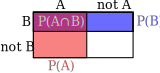
\includegraphics[width=0.7\textwidth]{figs/cosmological_parameters/bayes_theorem.pdf}
  \end{center}
  \caption{Diagram for Bayes theorem.  The probability for event A is in red and the probability for event B is in blue.  These overlap to form purple in the region of the probability of both events occuring jointly.}
\end{figure}


\begin{equation}
  P(A|B) = \frac{P(A\cap B)}{P(B)}
\end{equation}
      
\begin{equation}
  P(A|B) P(B) = P(A \cap B) =   P(B|A) P(A)
\end{equation}


posterior probability
likelihood
prior probability


\subsection{Gaussian likelihood in the case of supernovae}




\subsection{Markov Chain Monte Carlo}

\subsubsection{Detailed Balance}

\subsubsection{Metropolis-Hastings algorithm}

\subsubsection{Affine invariant algorithm}
emcee \citep{2013PASP..125..306F}


\chapter{Correlation functions and power spectra}

Although we live in a three-dimensional space, we will introduce concepts of harmonic analysis in one dimension for simplicity.  This has applications to measurements of the density along lines of sight, like absorption of Lyman-$\alpha$ in quasar spectra.  We can then generalize to harmonics in two dimensions on the sky and three dimensions filling all space.

To be general, we will represent density, absorption, emission of whatever we are representing as a function $a(x)$ of the comoving position $x$.

\section{Correlation function}





\section{Power spectra}
It has a fourier decomposition
\begin{equation}
  a(x) = \int \frac{dk}{2\pi}\ a(k) \exp(i kx) 
\end{equation}
so that the coefficients of the expansion are 
\begin{equation}
  a(k) = \int dx\ a(x) \exp(-i kx)
\end{equation}
These are called the harmonic coefficients at comoving wavenumber $k$.  They are the complex amplitudes of the (oscillatory, complex exponential) Fourier modes.%
%
\footnote{The convention in cosmology is to decompose large scale structure in flat space with modes like $\exp(i \mathbf{k} \cdot \mathbf{x})$.  The comoving wavenumber $k$ is like an angular frequency ($\omega$).  I agree with Numerical Recipes \citep{} that expressing the standard frequency as $f = \omega/2\pi$ makes the notation for Fourier transforms cleaner, but  we stick to the comoving wavenumber convention here.  If the space is not flat, $\exp(i \mathbf{k}\cdot \mathbf{x})$ is not correct basic to expand into, and we use other, more complicated, hypergeometric functions instead, which are the solutions to the wave equation in those spaces.}  Sometimes we will refer to $k$ as the (spatial) frequency.
The second equation is called the Fourier transform or analysis of the function, while the first is called the inverse fourier transform or the synthesis of the function.  We build up the function out of the oscillatory modes, and the harmonic coefficients tell us how much of each mode we need.

The definition of the power spectrum is the variance of the Fourier modes.
\begin{equation}
  \langle a(k) a^*(k') \rangle = 2\pi P(k) \delta(k - k') 
\end{equation}
This definition is extremely important and we will use it and similar relationships again and again.  For a homogeneous and isotropic signal, the different $k$ modes are independent, and 

Spectra are often classified as red, white, or blue, metaphorically named after the color of light with a similar spectral energy distribution.  Red spectra have more power at large scales, white spectra have equal power at all scale, and blue spectra have more power at small scales.

\subsection{Relationship between power spectrum and correlation function in 1d}




\subsection{Average correlation in a small interval}
How do we think about the infinity in correlation caused by the delta function?  This is linked to the fact that we are integrating here a statistically homogeneous function (one that never goes to zero) over an infinite volume.  But in practice, we will always be dealing with some interval in harmonic space that we can integrate the correlation over.  For example, if we have the transform, we can compute the average of the transform in a small interval $\Delta k$ in $k$-space
\begin{equation}
  \bar a(k) = \frac{1}{\Delta k} \int_{\Delta k} dk' a(k')
\end{equation}
Then we can examine the correlation of those fourier-space average quantities, as below, and see that they relate to the average power spectrum for that interval. 
\begin{eqnarray}
  \langle \bar a(k)  \bar a^*(k) \rangle &=& \frac{1}{(\Delta k)^2} \int_{\Delta_k} dk'_1 dk'_2 \langle a(k'_1) g^*(k'_2) \rangle \\
  &=& \frac{1}{(\Delta k)^2} \int_{\Delta k} dk'_1 dk'_2 \ 2\pi P(k'_1) \delta(k'_1 - k'_2) \\
  &=& \frac{2\pi}{(\Delta k)^2}  \int_{\Delta k} dk'_1 \  P(k'_1) \\
  &=& \frac{2\pi}{\Delta k}  \bar P(k),
\end{eqnarray}
where we are using the last equality to define what we mean exactly by average power.  Here we made sure the intervals over which we are averaging the harmonics are the same.  Otherwise, in distinct intervals the correlation would obviously be zero due to the delta function.


\section{Incomplete data}

We are always limited to the area of sky or volume of the universe we can access.  Additionally, if part of the signal is not available or of poor quality, we can downweight its importance or mask it out completely with a weight function $w(x)$.  This function would typically range from zero to one, giving no weight to bad data and full weight to good data.  Then the weighted signal
\begin{equation}\tilde a(x) = a(x) w(x)\end{equation}
has fourier components
\begin{equation}
  \tilde a(k) = \int dx\  \exp(-i k x) a(x) w(x).
\end{equation}
These are call the \textit{pseudo-}harmonics.

If we want to compute the correlation or pseudo-power spectrum from these weighted harmonics, we can just start expanding according to the definition of the harmonics.
\begin{eqnarray}
  \langle \tilde a(k) \tilde a^*(k') \rangle = &\int& dx dx' \ \exp(-i k x)\exp(i k' x') \langle a(x) a^*(x') \rangle w(x) w(x')  \nonumber \\
  = &\int &dx dx' \ \exp(-i k x)\exp(i k' x')  \nonumber \\
  & & \frac{dk_1}{2\pi} \frac{dk_2}{2\pi} \exp(i k_1 x)\exp(-i k_2 x')  \nonumber \\
  & & \langle a(k_1) a^*(k_2) \rangle w(x) w(x')  
\end{eqnarray}
Note the expansion of the complex conjugate of $a(x')$, which is real valued and so equals the conjugate.
 \begin{eqnarray}
   \langle \tilde a(k) \tilde a^*(k') \rangle  &= \int &dx dx' \ \exp(-i k x)\exp(i k' x')  \nonumber \\
  & &\frac{dk_1}{2\pi} \frac{dk_2}{2\pi} \exp(i k_1 x)\exp(-i k_2 x')  \nonumber \\
  & & 2\pi \delta(k_1 - k_2) P(k_1) w(x) w(x') 
\end{eqnarray}
Now we integrate the delta function over $k_2$ and collect the exponential functions of $x$ and $x'$ each together.
 \begin{eqnarray}
   \langle \tilde a(k) \tilde a^*(k') \rangle  &= & \int\frac{dk_1}{2\pi} dx dx' \ \exp(-i (k - k_1) x)\exp(i (k'-k_1) x')  \nonumber \\
  & &  \nonumber \\
   & &  w(x) w(x') P(k_1) \nonumber \\
   &=&  \int\frac{dk_1}{2\pi} \left[  w(k-k_1) w^*(k'-k_1) \right] P(k_1) %\nonumber \\
%   &=&  \int\frac{dk_1}{2\pi}  W(k_1-k) P(k_1)
\end{eqnarray}
using the definition of the fourier transform of the weight $w$ in the last step.  This is saying that, on average, the correlation of the masked signal is the convolution of the power spectrum with some kernel (in brackets) based on the mask or weighting function.  We will see a similar result below for more realistic and discretely sampled data.

\section{Discrete data}

In practice we have sampled data $a_j = a(x_j)$ where $x_j = j\Delta x$ is sampled at intervals $\Delta x = L/N$, where the total interval runs from $x=0$ to $x=L$ and is split into $N$ samples.  We assume that the function is periodic on that interval.  Then the Fourier transform integral becomes a Riemann sum.


We can compute the transform using intervals in harmonic space $k_p = p\Delta k$ where the interval size $\Delta k = 2\pi/N\Delta x$.  Every sample gets a position index $j$ and every harmonic gets a frequency index $p$.
\begin{eqnarray}%%%
  a_p = a(k_p) & = & \Delta x \sum_j a(t_j) \exp(- i k_p  x_j) \\
  & = & \Delta x \sum_j a_j \exp(-2\pi i pj/N). \label{eqn:dft}
\end{eqnarray}
 This sum is in the form of a discrete fourier transform.  This is very advantageous because computer algorithms can compute this very fast: the Fast Fourier Transform (FFT) algorithm can use divide-and-conquer techniques to compute the $N$ results in ${\cal O}(N \log N)$ operations instead of ${\cal O}(N^2)$, which is what a naive implementation would take.  At large sizes, this is a significant computational savings.

 Similarly, we can synthesize a discrete time series from Fourier coefficients as
 \begin{eqnarray}
   a_j = a(x_j) = \frac{\Delta k}{2\pi}  \sum_p a_p \exp(2\pi i pj/N) \label{eqn:idft}
 \end{eqnarray}

 ***Say something about the exact result versus approximate Riemann sum, nyquist frequency up-down-up-down $k_{\rm max} = k_{\rm Ny} = \pi / \Delta x$.  Band limit and aliasing.

 
 The definition of the power spectrum here is
 \begin{equation}
   \langle a(k_p) a^*(k_{p'}) \rangle = 2\pi \bar P(k_p) \frac{\delta_{pp'}}{\Delta k} \label{eqn:power_spectrum_definition_discrete}
  \end{equation}
 coming from the earlier equation for the average power in a small cell.  The kronecker delta scaled by the cell in fourier space takes the place of the dirac delta function in the original definition.  We'll drop the bar on $P$ for the upcoming discussion.

\subsection{Implementation and synthetic signals}
On a computer, the signal that we are trying to transform is often a real-valued array of numbers (and less often a complex array).  We have played a little fast and loose with the limits on the indices, which will correspond to the array in the computer, but we need to be careful to get things right.

In the Riemann sums, if we include the left side of every interval, then the sum in Eq.~\ref{eqn:dft}, for example, should include position indices $j = 0 \dots N-1$.  We can compute positive and negative frequencies, so you could imagine letting the frequency index $p = -N/2 \dots N/2$.  However, it is also clear that Eq.~\ref{eqn:dft} is periodic in $p$ with period $N$, so $a_p = a_{p+N}$.  In particular, the negative frequencies can be remapped to positive frequencies: $a_{-p} = a_{N-p}$.  Thus most implementations will also let the range on frequency index be $p = 0 \dots N-1$, similar to the position index.

In this convention, the zero frequency is stored at $p=0$.  Then the positive frequencies are stored in the first half of the array, at $p=1 \dots \lfloor N/2 \rfloor -1$.  The the negative frequencies start at $p =  \lfloor N/2 \rfloor$ and are placed in increasing order up to $p = N-1$, which holds frequency $-\Delta k$ in the very last array entry.  In higher-dimension FFTs, we follow this convention for all the frequency indices.

Some computer libraries or packages will have a special FFT routine for real-valued signals.    Because a real function is its own complex conjugate, we have that $a(x)$ implies $a(-k) = a^*(k)$.  Thus, for a real function, the negative-frequency harmonics are the complex conjugates of the positive frequency harmonics.  To save space, these real-to-complex transform routines will use a real array of size $N$ for the signal and a complex array of size $\lfloor N/2 \rfloor - 1$ for the harmonics, saving about half on memory usage.  In higher-dimension FFTs, only one of the indices is treated this way, typically the index that changes the fastest as you step through memory.

Now we have all the tools to make a synthetic, real-valued signal whose power spectrum we specify.  After choosing what $P(k)$ we want for the power spectrum, and remembering that the power spectrum provides the variance for the harmonic coeffients, $ \langle a(k_p) a^*(k_{p'}) \rangle = 2\pi P(k_p) / \Delta k$, we can set the zero mode as
\begin{equation}
  a(k = p =0) =  \frac{2\pi}{\Delta k } P(k = 0)\, Z_1
\end{equation}
where $Z_1$ is a random variable with zero mean and unit variance.  Note that the zero harmonic must be real valued.  Almost always, we want to create a Gaussian random field, and so use a routine to generate $Z_1$ as a random deviate distributed from a normal distribution like $Z_1 \sim {\cal N}(\mu = 0, \sigma^2 = 1)$.

Next we loop through the positive and negative frequencies together, ensuring that the harmonics are set as complex conjugates and get the correct variance.  For each $p$, 
\begin{equation}
  a_p =  a^*_{N-p} = \frac{2\pi}{\Delta k } P(k = p \Delta k) \frac{Z_1 + i Z_2}{\sqrt{2}}
\end{equation}
where $Z_1$ and $Z_2$ are both unit-variance deviates.  We populate the real and imaginary part of the harmonic on equal footing and normalize with the $\sqrt{2}$ because the variance of the deviates is $\langle |Z_1 + i Z_2 |^2 \rangle = \langle Z_1^2\rangle + \langle Z_2^2  \rangle = 2$.

\subsection{Weighting and masking}
 Let us add a mask or weight function to the discretely sampled data, so the weighted data and harmonics are
 \begin{eqnarray}
   \tilde a_j &=& a_j w_j \\
   \tilde a_p &=& \Delta x \sum_j \exp(-2\pi i pj/N) a_j w_j
 \end{eqnarray}

 As a start to computing the correlation, we can take the product of the masked harmonics, and then expand the true signal into the true harmonics:
 \begin{eqnarray}
   |\tilde a_p |^2 = \tilde a_p \tilde a_p^* &=&  (\Delta x)^2 \sum_{jj'} \exp(-2\pi i pj/N) \exp(2\pi i pj'/N) a_j  a_{j'} w_j w_{j'}  \nonumber \\
   &=&  (\Delta x)^2 \sum_{jj'} \exp(-2\pi i pj/N) \exp(+2\pi i pj'/N) \nonumber \\
   & & \times   \left(\frac{\Delta k}{2\pi}\right)^2 \sum_{p_1 p_2}  \exp(2\pi i p_1 j/N) \exp(-2\pi i p_2 j'/N) \nonumber \\
   & & \times a_{p_1} a^*_{p_2} w_j w_{j'}
 \end{eqnarray}
Let's cancel the $\Delta x$ with the $\Delta k$ and take the ensemble average, using the Eq.~\ref{eqn:power_spectrum_definition_discrete} replace the product of harmonics.
 \begin{eqnarray}
 \langle  |\tilde a_p |^2 \rangle &=& \left(\frac{\Delta x\Delta k}{2\pi}\right)^2  \sum_{jj'p_1p_2} \exp(-2\pi i pj/N)  \exp(+2\pi i pj'/N) \nonumber \\
 & & \exp(2\pi i p_1 j/N) \exp(-2\pi i p_2 j'/N){2\pi} P(k_{p_1}) \frac{\delta_{p_1 p_2}}{\Delta k} w_j w_{j'}
 \end{eqnarray}
Use the delta function to sum over $p_2$ and separately gather the exponentials with $j$ and $j'$.  
\begin{eqnarray}
 \langle   |\tilde a_p |^2 \rangle &= \frac{\Delta k}{2\pi}\left(\Delta x \right)^2  \sum_{jj'p_1}& \exp(-2\pi i (p-p_1)j/N)  w_j \nonumber \\
  & &  \exp(+2\pi i (p-p_1) j'/N)  w_{j'}   P(k_{p_1})
\end{eqnarray}
That reveals Fourier tranforms of the weight functions
\begin{eqnarray}
  \langle  |\tilde a_p |^2 \rangle &=& \frac{\Delta k}{2\pi}  \sum_{p_1} w_{p-p_1} w_{p-p_1}^*  P(k_{p_1}) \\
  &=& \left(\frac{\Delta k}{2\pi}\right)  \sum_{p_1} |w_{p-p_1}|^2  P(k_{p_1})
\end{eqnarray}
Multiplying both sides by $2\pi/\Delta k$ we can define the observed pseudo-spectum as
\begin{equation}
  \tilde P(k_p) = \frac{2\pi}{\Delta k} |\tilde a_p |^2
\end{equation}
to obtain a statistic that is, on average, simply related to the true power spectrum. We can package the modulus of the weight function harmonics as a matrix,
\begin{equation}
  W_{pp_1} =  |w_{p-p_1}|^2,
\end{equation}
and express the whole relationship between the ensemble average of the observed pseudo power spectrum and the true spectrum as a matrix equation
\begin{equation}
  \langle \tilde P(k_p) \rangle =  \sum_{p_1} W_{pp_1}  P(k_{p_1})
\end{equation}
or written as a matrix equation
\begin{equation}
  \langle \tilde P \rangle =  W  P \label{eqn:ensemble_mode_coupling_matrix_times_power}
\end{equation}


This suggests to invert the $W$ matrix to get an unbiased estimate of the observed power spectrum as something like ``${P}^{\rm obs} = W^{-1} \tilde P$,'' and indeed this is our basic strategy, but there are some subtleties.  First, $W$ may be non-invertible.  There is no guarantee of it and the more of the data the mask removes, usually the harder it is to invert $W$.  Furthermore, the pseudo-spectrum $\tilde P$ only draws one sample of the power for the mode at $k_p$, so the sample variance is very large.  In the next section, we will find that binning together several modes with similar wavenumbers can help to alleviate both problems.

\section{Band powers}
To improve statistics on the estimation of the spectrum, we want to average together the power from several harmonics.  We will do this with a matrix ``binning operator'' $B$ that makes a weighted average of the power over some band of wavenumbers
\begin{equation}
  \tilde {\cal P}_b  = \sum_p B_{bp} \tilde P_p
\end{equation}
where the reduced-size, binned pseudo-spectrum is on the left and the band $b$ contains some set of harmonics.   We use weights $g(p)$ in the band, so that the total weight in a band is
\begin{equation}
  G(b) = \sum_{p\ {\rm in}\ b} g(p).
\end{equation}
We set up the binning operator with the total weight as the normalization to the weighted average
\begin{equation}
  B_{bp} = \left\{
  \begin{array}{ll}
   g(p)/G(b), &  \mbox{harmonic $p$ in band $b$} \\
   0, & \mbox{otherwise}
  \end{array} 
  \right.
\end{equation}
End band is disjoint: each harmonic contributes only to a single band.

We also need an ``unbinning'' operator $\bar B_{pb}$, or reciprocal binning operator, so that
\begin{equation}
  \sum_p B_{bp}\bar B_{pb'} = \delta_{bb'}  \label{eqn:binning_delta_function}
\end{equation}
It is the right-inverse of $B$.  That is saying that if you had a binned spectrum, unbinned it, and binned it back, it would be be unchanged.  However, we cannot go the other way.  The binned spectrum has less information in it than the unbinned spectrum, and we cannot recover details of the spectrum finer than the bin width once it has been binned.    An unbinning operator with this property is
\begin{equation}
  \bar B_{pb} = \left\{
  \begin{array}{ll}
   {h(p)/H(b)}, &  \mbox{harmonic $p$ in band $b$} \\
   0, & \mbox{otherwise}
  \end{array} 
  \right.
\end{equation}
so long as the normalization is 
\begin{equation}
  H(b) = \frac{1}{G(b)}\sum_{p\ {\rm in}\ b}g(p)h(p).
\end{equation}
In an exercise, you can show that this definition satisfies Eq. \ref{eqn:binning_delta_function}.  The function $h(p)$ is the anticipated shape of the power spectrum within the band.

We have freedom to choose whatever weights and power spectrum shape are most appropriate to our particular case, but in typical usage, we might choose uniform weights ($g(p) = 1$) and flat band powers ($h(p)=1$).  That choice sets $G(b)$ to be the count of harmonics contributing to the band and $H(b) = 1$.  In this typical usage, we end up assuming that the power spectrum is flat in the bands determined by the bins.

The matrix product
\begin{equation}
  \sum_b \bar B_{pb}B_{bp'} 
\end{equation}
is not the identity matrix, but, applied to a power spectrum, will average it into piecewise bands of the specified shape determined by $h(p)$.


\section{Estimated spectra, band power window functions}

Let's employ this binning, looking back at Eq.~\ref{eqn:ensemble_mode_coupling_matrix_times_power}, which says that the ensemble average of the pseudo-spectrum is the mode-coupling matrix times the true power spectrum.  Applying the binning operation to both sides using a matrix notation to make the math easier:
\begin{equation}
  B \langle \tilde P \rangle =  B W  P
\end{equation}
Then we approximate $\bar B B$ as the identity matrix and insert it between the mode-coupling matrix and the true spectrum.
\begin{equation}
  B \langle \tilde P \rangle \approx  B W {\bar B} B P. \label{eqn:bandpower_approximation}
\end{equation}
This is only exact if the power spectrum $P$ has the same functional form as anticipated in the reciprocal binning operator.  Then we can invert the binned mode-coupling matrix and bring everything inside the ensemble average to obtain
\begin{equation}
 \langle( B W {\bar B})^{-1} B \tilde P \rangle \approx B P
\end{equation}

Thus we define our observed power spectrum as the quantity inside the average
\begin{equation}
{\cal P^{\rm obs}} \equiv ( B W {\bar B})^{-1} B \tilde P 
\end{equation}
to get something that is approximately equal (on average) to the binned true power spectrum.  We also define the binned  mode coupling kernel
\begin{equation}
  K_{bb'} =  B_{bp} W_{pp'} \bar B_{p'b'}.
\end{equation}
This binned mode coupling matrix may be invertible even when the unbinned matrix is not.

We use the matrix inverse to decouple the binned pseudo-powerspectrum to get an estimated or observed power spectrum.
\begin{equation}
  {\cal P}^{\rm obs}_b = \sum_{b'} \left( K^{-1} \right)_{bb'} \tilde {\cal P}_{b'} 
\end{equation}

What if we want to correct for the approximation in Eq.~\ref{eqn:bandpower_approximation}?  
Using a matrix notation again, we can relate the ensemble average of the observed power spectrum (${\cal P}^{\rm obs}$) to the average of the binned pseudo-spectrum ($\tilde {\cal P}$), and then to true power spectrum of the signal ($P$).
\begin{eqnarray}
  \langle {\cal P}^{\rm obs} \rangle &=& K^{-1} \langle \tilde {\cal P} \rangle \\
  &=&  (B W \bar B)^{-1} B W P \\
\end{eqnarray}
We define the \textit{band power window function} (${\cal W}_{bp}$), defined by the matrix equation
\begin{equation}
  {\cal W} = (B W \bar B)^{-1} B W,
\end{equation}
 so that
\begin{equation}
  \langle {\cal P}^{\rm obs} \rangle = {\cal W} P
\end{equation}
It relates the the contribution of a true power spectrum to the (binned and decoupled) bandpower estimate of the observed power spectrum.  This is important for comparing theory to data.  Any particular theory prediction for $P(k)$, operated on my the band power window function, is the prediction for the average value of the oberserved power spectrum ${\cal P}^{\rm obs}_b$.

\section{Signal, noise, and cross-spectrum}

\nocite{numerical_recipes,master,namaster}


\section*{Exercises}

\begin{enumerate}

\item Show that homogeneity implies that the modes are independent.

\item Compute the pseudo power spectrum of a signal that has a white-noise power spectrum.

\item Show that $B\bar B$ is the identity matrix.

\item Show that $P = \bar B B P$ is only true when $P$ is (piecewise) proportional to $h(p)$.  (It is sufficient to show it for some generic bin $b$.)
  
\end{enumerate}


\section*{Supplemental: Dirac delta functions}
The important property of the Dirac delta function are
\begin{equation}
  \int_{\Delta x} dx'\ \delta(x-x') = \left\{
  \begin{array}{ll} 1, & \mbox{if $x$ is in $\Delta x$;} \\ 0, & \mbox{otherwise.} \end{array}
  \right.
\end{equation}
Integrated (really convolved) against a function, the Dirac delta function selects a function value as so:
\begin{equation}
  \int dx'\ \delta(x-x') f(x') = f(x)
\end{equation}

The Dirac delta function is also the Fourier transform of the constant unit function.
\begin{equation}
   \delta(x-x') = \int \frac{dk}{2\pi} \exp(i k (x-x')) 
\end{equation}
On the right side, it is clear that if $x=x'$, the exponential equals one and the integral over the whole real line is infinity.  On the other hand, if $x \neq x'$, the integrand is oscillatory and will not diverge.  You can integrate over this Fourier definition of the delta function over some interval containing $x$ or not to show that it produces the expected values.  We can write a similar defition for the fourier transform of the $k$-space delta function by swapping names of the $x$ and $k$ variables.
\begin{eqnarray}
  \delta(k - k') &=& \frac{1}{2\pi}  \int {dx}\ \exp(i (k-k')x)    \\
  &=& \frac{1}{2\pi}  \int {dx}\ \exp(-i (k'-k)x) 
\end{eqnarray}
where we are careful with the minus sign in the last equation to match up with our definition of inverse Fourier transform.  The dirac delta function is even ($\delta(k-k') = \delta(k' - k)$) and real valued (equal to its complex conjugate, replacing $i$ with $-i$), so there are lots of variations of minus signs that are equivalent.  Take some care with them.

\chapter{The Cosmic Microwave Background}

What is the cosmic microwave background?

The universe is not perfectly homogeneous, but the perturbations are small at early times and on large scales.


The CMB power spectrum is pillar of modern cosmology because it is both measureable and predictable from theory.

T = 0.3 eV atoms form

T = 0.25 eV photons decouple and stream freely

z = 1100

$t_{\rm CMB} = $ 380,000 years


\section{Anisotropies}
To examine correlations in the CMB we again want to decompose it into a series of harmonic functions.  Because the surface of the sphere has a finite area, the spectrum of harmonics is discrete.  We can write it as
\begin{equation}
  T(\mathbf{n} = \theta,\phi) = \sum_{lm} a_{lm} Y_{lm}(\mathbf{n})
\end{equation}
where the $Y_{lm}$ functions are the spherical harmonic functions and the $a_{lm}$ is common name for the harmonic coefficients.  Most of the time, the exact form of these functions are not important, but we sometimes use some definitions and identities that are listed in a supplemental section at the end of this chapter.

As usual, the power spectrum (typically called $C_l$) is the variance of the harmonic coeffients.  The $a_{lm}$ are statistically independent, and so the covariance matrix of them is diagonal.  We express this as
\begin{equation}
  \langle a_{lm} a_{l'm'}^* \rangle = C_l \delta_{ll'} \delta_{mm'}
\end{equation}
Using a Boltzmann solver, we can compute this theoretical power spectrum from a particular cosmological model via the parameters $C_l(\Omega_c,\Omega_b,\dots)$.  

The CMB is very Gaussian.  In other words, each complex-valued $a_{lm}$ is drawn from a Gaussian distibution with mean zero and variance $C_l$.  Because the temperature is real valued,  $a_{l(-m)} = a_{lm}^*$ and the positive $m$-values determine the negative ones. Every $m$ value for the same $l$ has the same variance, so a simple estimator for the power spectrum is to average over the different $m$s,
\begin{equation}
  \bar C_l = \frac{1}{2l+1} \sum_m |a_{lm}|^2,
\end{equation}
but this type of estimator is biased if the whole sky is not available.


\section{What information is in the power spectrum?}


\section{Signal, beam, pixels, and noise}

The CMB signal is smoothed by the finite resolution of the telescope.  We describe the point-spread function or the beam of the telescope by a function on the sphere $b(\mathbf{n})$ which is mostly concentrated around its maximum at the north pole but can have sidelobes caused by diffraction into the aperture.  The actual temperature that the telescope sees at an instant can be expressed as a convolution
\begin{equation}
  T(\mathbf{n},\omega) = \int d\mathbf{n}' [D(\mathbf{n},\omega)b](\mathbf{n}') T(\mathbf{n}')
\end{equation}
The rotation operator $D$ takes the beam from its fiducial orientation to point in the direction $\mathbf{n}$ with an orientation rotation $\omega$ around the telescope boresight, then the integral collects the light from the unmodified sky in the directions that the telescope is sensitive to.  Unlike optical telescope, CMB telescopes do not take pictures.  They scan back and forth over and over, collecting low signal-to-noise data that is later averaged and re-assembled into a sky map.  We defer the mapmaking discussion to later, but one consequence is that one point on the sky may be seen from many different angles and by many different detectors, which can average to symmetrize the beam.  So although there are fast algorithms to compute the full convolution\footnote{totalconvolver}, for the main beam, it is often good enough to use a azimuthally symmetric beam approximation $b(\mathbf{n}) = b(\theta)$.  In that case the beam convolution can be written as a multiplication in harmonic space,
\begin{equation}
  a_{lm}^{\rm beam} = b_l a_{lm}
\end{equation}


\begin{equation}
  b_l = \int d(\cos \theta) P_l(\cos \theta) b(\theta)
\end{equation}

The signal on the sky has units like spectral flux density per solid angle, for example Jy/sr.  An extended source of radiation, like a dust cloud in the Milky Way, nearby galaxy large enough to see detail, or the Cosmic Microwave Background (CMB) also has a \textit{surface brightness} given in the same units, and by integrating over an aperture, you can measure how much total brightness (flux density) an object has.



pixel window function


Noise

red at low multipoles, white at high multipoles

$l_{\rm knee}$

The total data 
\begin{equation}
  a^{\rm data}_{lm} = b_l a_{lm} + n_{lm}
\end{equation}
fits the model of data equals response to signal plus noise.




\section{Measuring the power spectrum}

two dimensional masking



including cross spectra


construction of the covariance matrix via cross spectra

errors, knox formula


\section{Time-ordered data, calibration, and mapmaking}

Planck satellite calibration on dipole and orbital changes to the dipole.

gain calibration

detector time constants; time constant deconvolution

deglitching

data cuts

filter and bin map making

maximum likelihood mapmaking

gain fluctuations model error


\section{Foreground mitigation}


\section{Likelihood construction}

full pixel-based likelihood

cross-spectra likelihood

early 2000s polarization likelihood whose name I'm blanking on...


\section{Polarization anisotropies}

\section{The flat-sky approximation}


\section*{Supplemental: spherical harmonic functions}

The function is band limited if there are only zero harmonics above some $l_{\rm max}$.  The CMB is not band limited, but our observation of the CMB is in practice band limited by the finite resolution of the telescope we use to observe it.

The spherical harmonics are complex functions
\begin{equation}
  Y_{lm}(\theta,\phi) = (-1)^m \sqrt{\frac{2 l + 1}{4\pi} \frac{l-m}{l+m}} P_l^m(\cos \theta) \exp(im\phi)
\end{equation}
that depend on the associated Legendre polynomials $P_l^m$.  In cosmology we use the same conventions that are common in quantum mechanics, in particular placing the factor of $(-1)^m$ (``Condon-Shortley'' phase) in the definition of the spherical harmonics and not in the definition of the associated Legendra polynomicals.

These functions have several important identities.  They are orthonormal functions integrated over the on the whole sphere
\begin{equation}
  \int d\Omega Y_{lm}(\theta,\phi) Y_{l'm'}(\theta,\phi) = \delta_{ll'} \delta_{mm'}
\end{equation}
This in particular means that for $l=0$, $m=0$, we must have
\begin{equation}
  Y_{00} = \frac{1}{(4\pi)^{1/2}}
\end{equation}

Another important identity for spherical harmonics is the addition theorem
\begin{equation}
  \sum_{m} Y_{lm}(\mathbf{n}) Y_{lm}(\mathbf{n}') = \frac{2l+1}{4\pi} P_l(\mathbf{n \cdot n}') 
\end{equation}
for $\mathbf{n}$ as a unit vector pointing to $(\theta,\phi)$ and similarly for $\mathbf{n}'$.




Expansion of a plane wave:
\begin{equation}
  \exp({i \mathbf k \cdot \mathbf r}) = \sum_{l} (2 l + 1) i^l j_l(k r) P_l(\hat{\mathbf k} \cdot \hat{\mathbf r})
\end{equation}
where $j_l$ are the spherical bessel functions of the first kind.

\begin{equation}
  \exp({i \mathbf{k} \cdot \mathbf{r}}) = 4 \pi \sum_{lm} i^l j_l(k r) Y_{lm}{}(\hat{\mathbf k}) Y_{lm}^{*}(\hat{\mathbf r})
\end{equation}
This relationship is vital when we come to projecting the harmonics of signal in the bulk of space into signals on the sphere of the sky.

\chapter{Filters and Secondary Anisotropies}


\section{Wiener filter}



\section{Matched filter}

\subsection{point sources}

\subsection{SZ and galaxy clusters}


\section{Lensing reconstruction}

\chapter{Galaxy correlations}

Perturbations in the matter field are small at early times and even today on large scales.  We can do perturbation theory and linearize the force of gravity.

\begin{equation}
\rho(\mathbf{x},t) = \bar \rho(t) + \delta \rho   (\mathbf{x},t)
\end{equation}
split the mean density from the density perturbation.

Over density perturbation
\begin{equation}
  \delta(\mathbf{x},t) = \frac{\delta \rho}{\rho} = \frac{\rho(\mathbf{x},t) - \bar \rho(t)}{\bar \rho(t)}
\end{equation}

Fourier expansion in flat space
\begin{equation}
\delta(\mathbf{x},t) = \int \frac{d^3k}{2\pi} \exp(i \mathbf{k \cdot x}) \delta(\mathbf{k},t) 
\end{equation}
We have the comoving vector $\mathbf{x}$ and the comoving wavevector  $\mathbf{k}$.  The wavenumber $k = | \mathbf{k} | = 2\pi/\lambda $ relationship to the comoving wavelength of the sinusoidal perturbation.

For non-flat spaces, $\exp(i \mathbf{k \cdot x})$ is the wrong basis function, but there are correct ones you can use if needed.

Once GR is linearized, the Fourier modes evolve independently following a differential equation
\begin{equation}
  \ddot \delta(\mathbf{k},t) + 2 H \dot \delta(\mathbf{k},t) + \left( \frac{c_s(t)^2 k^2}{a^2} - 4\pi G \bar \rho(t) \right) \delta(\mathbf{k},t)
\end{equation}
Depending on the signs of the terms, this looks an equation for a damped harmonic oscillator or for an unstable exponential growth or decay.

In the second term, the Hubble parameter looks like the damping term in the oscillator equation and is referred to the Hubble friction.  It corresponds to expansion damping the growth of perturbation by spreading material out.  In the first part of the third term, the pressure term retards growth as the pressure of the fluid resists collapse.  In the second part of the third term, gravity promotes growth.

Early on the sound speed is for a relativistic fluid.  \textbf{At late times, I don't know if there is an effective k dependence in the sound speed.  Probably.}

Growth functions on large scales
solutions
\begin{equation}
   \delta(\mathbf{k},t) =  \delta_+(\mathbf{k}) D_+(t) + \delta_-(\mathbf{k}) D_-(t)
\end{equation}
ignore the decaying modes.

Growing modes have different behavior inside and outside the horizon which gives rise to the overall shape of the matter power spectrum.

The matter power spectrum is
\begin{equation}
\langle  \delta(\mathbf{k}) \delta^*(\mathbf{k'}) \rangle = (2\pi)^3 P(k) \delta(\mathbf{k-k'})
\end{equation}

Galaxies are biased tracers of the matter field.  Typically this is modeled with a linear bias, e.g. for galaxies of mass $M$
\begin{equation}
  \delta_g(\mathbf{k}) = b(M) \delta(\mathbf{k}).
\end{equation}
More massive galaxies tend to form in denser areas, at the peaks of the density field, and so are are more biased.

\begin{figure}
  \begin{center}
    \fakeplot
  \end{center}
  \caption{Plot showing the increase in bias as a function of mass.}
\end{figure}

The relationship between a power spectrum and a correlation function is
\begin{equation}
  A(\mathbf{x}) = \int \frac{d^3k}{(2\pi)^3} \exp(i \mathbf{k \cdot x}) A(\mathbf{k})
\end{equation}
\begin{eqnarray}
  \langle A(\mathbf{x})A(\mathbf{x}')^*\rangle &=& \int \frac{d^3k}{(2\pi)^3}\frac{d^3q}{(2\pi)^3} \exp(i \mathbf{k \cdot x}) \exp(-i \mathbf{q \cdot x'}) \langle A(\mathbf{k}) A(\mathbf{q})^* \rangle \\
  &=&  \int \frac{d^3k}{(2\pi)^3}\frac{d^3q}{(2\pi)^3} (2\pi)^3 P(k) \delta(\mathbf{k-q}) \exp( i \mathbf{k \cdot x} -  i \mathbf{q \cdot x'}) \\
  &=& \int \frac{d^3k}{(2\pi)^3}  P(k) \exp(i \mathbf{k \cdot (x-x')}) \\ 
\end{eqnarray}

\begin{equation}
 \langle  A(\mathbf{x})A(\mathbf{x+r}) \rangle = \frac{4\pi}{(2\pi)^3} \int dk\, k^2\, \frac{\sin(kr)}{kr} P(k)
\end{equation}

\section{Baryon Acoustic Oscillations}


\section{Correlation functions}
\section{Power spectra}
\section{Alcock-Paczynski test}



\section*{Supplemental: Fourier transform of a spherical function}
\begin{eqnarray}
  f(\mathbf{k}) &=& \int d^3x \exp(- i \mathbf{k \cdot x}) \\
  &=& \int d^3x \exp(- i \mathbf{k \cdot x}) Y_{00} \sqrt{4\pi}
\end{eqnarray} 

\chapter{Gravitational lensing and cosmic shear}


\section{Intrinsic alignments}
NLA model (nonlinear alignment model)

\chapter{Cross-correlations}

Cross correlation are a good way to measure halo bias, the growth of structure, and the overall amplitude of fluctuations.

tomographic

Fluctuations amplitudes $S_8 = \sigma_8 (\Omega_m /0.5)^{0.5}$

autocorrelation together with lensing breaks the bias degeneracy

stacking
cross-correlation function
cross power spectrum

\section{Synthesizing cross-correlations}


At each multipole $l$
\begin{equation}
  C_l = \left( \begin{array}{cccc}
    C^{aa} & C^{ab} &  C^{ac} &  \\
    C^{ba} & C^{bb} &  C^{bc} & \dots \\
    C^{ca} & C^{cb} &  C^{cc} &  \\
    & \vdots & & \ddots
  \end{array} \right)_l
\end{equation}

Since as a covariance this is a real, positive definite, symmetry array, it has a Cholesky decomposition
\begin{equation}
  C_l = LL^\dag
\end{equation}

mix the alms
\begin{equation}
  a_{i,lm} =\sum_j L_{ij,l} Z_{j,lm}
\end{equation}


\section{Limber approximation}



\section{Computing cross correlations}

contamination
interlopers

jackknife error bars

\chapter{Nonlinearities}
\section{Halo model}
\section{Lognormal model}
\section{$N$-body simulations}


\bibliographystyle{apj}
\bibliography{ref.bib}
 
\printindex

 

\end{document}
